\documentclass[a4paper,10pt,titlepage]{scrbook}

% project information
\newcommand{\TITLE}{SMT-RAT}
\newcommand{\VERSION}{0.4.0}

\usepackage{amssymb,amsmath} % math symbols
\usepackage{amstext}
\usepackage{tikz} % draw graphs and many more
\usepackage{color}
\usepackage{xspace}
\usepackage{hyperref}
\usepackage{verbatim}
\usepackage{enumerate}
\usepackage{float}
\floatstyle{boxed} 
\restylefloat{figure}


% Listings setting
%\lstset{language=C++,frame=single,morekeywords={RationalUnivariatePolynomial,ex,symbol,pow,list,IntervalRepresentation,invalid_argument}}

% Search path for pictures

\newcommand{\automake}{\href{http://www.gnu.org/software/automake/}{\texttt{automake}}\xspace}
\newcommand{\automakeURL}{\href{http://www.gnu.org/software/automake/}{\color{blue}http://www.gnu.org/software/automake/}\xspace}
\newcommand{\cmake}{\href{http://www.cmake.org/}{\texttt{cmake}}\xspace}
\newcommand{\cmakeURL}{\href{http://www.cmake.org/}{\color{blue}http://www.cmake.org/}\xspace}
\newcommand{\ccmake}{\href{http://www.cmake.org/}{\texttt{ccmake}}\xspace}
\newcommand{\java}{\href{http://openjdk.java.net/}{\texttt{java}}\xspace}
\newcommand{\javaURL}{\href{http://openjdk.java.net/}{\color{blue}http://openjdk.java.net/}\xspace}
\newcommand{\gplusplus}{\href{http://gcc.gnu.org/}{\texttt{g++}}\xspace}
\newcommand{\gplusplusURL}{\href{http://gcc.gnu.org/}{\color{blue}http://gcc.gnu.org/}\xspace}
\newcommand{\B}{\ensuremath{\mathbb{B}}\xspace}
\newcommand{\true}{\ensuremath{\texttt{true}}\xspace}
\newcommand{\false}{\ensuremath{\texttt{false}}\xspace}
\newcommand{\formula}{\ensuremath{\textit{Formula}_{RA}}\xspace}
\newcommand{\prop}{\ensuremath{\textit{Prop}}\xspace}
\newcommand{\strategy}{\ensuremath{\textit{Strat}}\xspace}
\newcommand{\Gentoo}{\href{http://www.gentoo.org/}{Gentoo Linux}\xspace}
\newcommand{\SMTRAT}{\href{http://smtrat.sourceforge.net/}{\texttt{SMT-RAT}}\xspace}
\newcommand{\Matlab}{\href{http://www.mathworks.de/}{\texttt{MATLAB}}\xspace}
\newcommand{\Mathematica}{\href{http://www.wolfram.com/}{\texttt{Mathematica}}\xspace}
\newcommand{\Synaps}{\href{http://www-sop.inria.fr/galaad/logiciels/synaps/}{\texttt{SYNAPS}}\xspace}
\newcommand{\Parigp}{\href{http://pari.math.u-bordeaux.fr/}{\texttt{PARI/GP}}\xspace}
\newcommand{\Kant}{\href{http://www.math.tu-berlin.de/~kant/kash.html}{\texttt{KANT}}\xspace}
\newcommand{\Singular}{\href{http://www.singular.uni-kl.de}{\texttt{Singular}}\xspace}
\newcommand{\Givaro}{\href{http://ljk.imag.fr/CASYS/LOGICIELS/givaro/}{\texttt{Givaro}}\xspace}
\newcommand{\Redlog}{\href{http://redlog.dolzmann.de/}{\texttt{Redlog}}\xspace}
\newcommand{\QEPCAD}{\href{http://www.usna.edu/Users/cs/qepcad/B/QEPCAD.html}{\texttt{QEPCAD}}\xspace}
\definecolor{ginac}{HTML}{BD0000}
\newcommand{\ginac}{{\texttt{GiNaC}}\xspace}
\newcommand{\Ginac}{\href{http://www.ginac.de/}{\texttt{GiNaC}}\xspace}
\newcommand{\ginacURL}{\href{http://www.ginac.de/}{\color{blue}http://www.ginac.de/}\xspace}
\newcommand{\cln}{{\texttt{cln}}\xspace}
\newcommand{\Cln}{\href{http://www.ginac.de/}{\texttt{cln}}\xspace}
\newcommand{\clnURL}{\href{http://www.ginac.de/}{\color{blue}http://www.ginac.de/}\xspace}
\newcommand{\carl}{{\texttt{carl}}\xspace}
\newcommand{\Carl}{\href{http://carl.sourceforge.net/}{\texttt{carl}}\xspace}
\newcommand{\carlURL}{\href{http://carl.sourceforge.net/}{\color{blue}http://carl.sourceforge.net/}\xspace}
\newcommand{\Cpp}{\texttt{C++}\xspace}
\newcommand{\Cppeleven}{\texttt{C++11}\xspace}
\newcommand{\Java}{\texttt{Java}\xspace}
\newcommand{\Reduce}{\href{http://www.reduce-algebra.com/}{\texttt{Reduce}}\xspace}
\newcommand{\Libreduce}{\href{http://www.reduce-algebra.com/}{\texttt{Libreduce}}\xspace}
\def\cocoa{{\hbox{\rm C\kern-.13em o\kern-.07em C\kern-.13em o\kern-.15em A}}}
\newcommand{\Cocoa}{\href{http://cocoa.dima.unige.it/}{\texttt{CoCoA}}\xspace}
\newcommand{\CocoaLib}{\href{http://cocoa.dima.unige.it/}{\texttt{CoCoALib}}\xspace}
\newcommand{\Maple}{\href{http://www.maplesoft.com/}{\texttt{Maple}}\xspace}
\newcommand{\Cppunit}{\href{http://sourceforge.net/projects/cppunit/}{\texttt{CppUnit}}\xspace}
\newcommand{\ginacra}{\href{http://ginacra.sourceforge.net/}{\texttt{GiNaCRA}}\xspace}
\newcommand{\ginacraURL}{\href{http://ginacra.sourceforge.net/}{\color{blue}http://ginacra.sourceforge.net/}\xspace}
\newcommand{\manualURL}{\href{http://smtrat.sourceforge.net/manual/manual.pdf}{http://smtrat.sourceforge.net/manual/manual.pdf}\xspace}
\newcommand{\smtrat}{\texttt{SMT-RAT}\xspace}
\newcommand{\smtratURL}{\href{http://smtrat.sourceforge.net/}{http://smtrat.sourceforge.net/}\xspace}
\newcommand{\ZThree}{\href{http://research.microsoft.com/en-us/um/redmond/projects/z3/}{\texttt{Z3}}\xspace}
\newcommand{\Cvc}{\href{http://cs.nyu.edu/acsys/cvc3/}{\texttt{CVC3}}\xspace}
\newcommand{\hysat}{\href{http://hysat.informatik.uni-oldenburg.de/}{\texttt{HySAT}}\xspace}
\newcommand{\absolver}{\href{http://absolver.sourceforge.net/}{\texttt{ABsolver}}\xspace}
\newcommand{\isat}{{\texttt{iSAT}}\xspace}
\newcommand{\minismt}{\href{http://cl-informatik.uibk.ac.at/software/minismt/}{\texttt{MiniSmt}}\xspace}
\newcommand{\sep}{\ensuremath{~\mid~}}
\newcommand{\R}{\ensuremath{\mathbb{R}}\xspace}
\newcommand{\formulaClass}{\texttt{Formula}\xspace}
\newcommand{\moduleClass}{\texttt{Module}\xspace}
\newcommand{\gbModuleClass}{\texttt{GroebnerModule}\xspace}
\newcommand{\vsModuleClass}{\texttt{VSModule}\xspace}
\newcommand{\lraModuleClass}{\texttt{LRAModule}\xspace}
\newcommand{\satModuleClass}{\texttt{SATModule}\xspace}
\newcommand{\cnferModuleClass}{\texttt{CNFerModule}\xspace}
\newcommand{\cadModuleClass}{\texttt{CADModule}\xspace}
\newcommand{\managerClass}{\texttt{Manager}\xspace}
\newcommand{\strategyClass}{\texttt{Strategy}\xspace}

\newcommand{\PREM}{\texttt{M$_\text{PRE}$}\xspace}
\newcommand{\CNFM}{\texttt{M$_\text{CNF}$}\xspace}
\newcommand{\SATM}{\texttt{M$_\text{SAT}$}\xspace}
\newcommand{\LRAM}{\texttt{M$_\text{LRA}$}\xspace}
\newcommand{\VSM}{\texttt{M$_\text{VS}$}\xspace}
\newcommand{\CADM}{\texttt{M$_\text{CAD}$}\xspace}
\newcommand{\GBM}{\texttt{M$_\text{GB}$}\xspace}

\newcommand{\CADModule}{\texttt{MC$_M$}\xspace}
\newcommand{\vsModule}{\texttt{VS$_M$}\xspace}
\newcommand{\groebnerModule}{\texttt{GS$_M$}\xspace}

\newcommand{\opensmt}{\texttt{OpenSMT}\xspace}
\newcommand{\Opensmt}{\href{http://verify.inf.usi.ch/opensmt}{\texttt{OpenSMT}}\xspace}
\newcommand{\opensmtURL}{\href{http://verify.inf.usi.ch/opensmt}{\color{blue}http://verify.inf.usi.ch/opensmt}\xspace}
\newcommand{\opensmtSMTRAT}{\texttt{Rat$_1$}\xspace}
\newcommand{\opensmtSMTRATGB}{\texttt{Rat$_2$}\xspace}
\newcommand{\opensmtSMTRATNoSimp}{\texttt{opensmtSMTRAT\_NoSimp}\xspace}
\newcommand{\zthree}{\texttt{Z3}\xspace}
\newcommand{\opensmtRedlog}{\texttt{opensmtRedlog}\xspace}
\newcommand{\opensmtRedlogNoSimp}{\texttt{opensmtRedlog\_NoSimp}\xspace}
\newcommand{\redlog}{\texttt{redlog}\xspace}
\newcommand{\redlogNoSimp}{\texttt{redlog\_NoSimp}\xspace}
\newcommand{\cvc}{\texttt{CVC3}\xspace}
\newcommand{\SAT}{\texttt{sat}\xspace}
\newcommand{\UNSAT}{\texttt{unsat}\xspace}
\newcommand{\UNKNOWN}{\texttt{unknown}\xspace}
\newcommand{\Crcv}{\ensuremath{C_{rcv}}\xspace}
\newcommand{\Cpass}{\ensuremath{C_{pas}}\xspace}
\newcommand{\Cinf}{\ensuremath{C_{inf}}\xspace}
\newcommand{\True}{\texttt{true}\xspace}
\newcommand{\False}{\texttt{false}\xspace}
\newcommand{\smtratLogic}{non-linear real and integer arithmetic with uninterpreted functions}
\newcommand{\SmtratLogic}{UF$\_$NRIA~}




\begin{document}

\begin{titlepage}
	\begin{center}
		\Huge{\textbf{\TITLE}}\\
		\Huge{Version \VERSION}\vspace{1cm}\\
		\Large Open Source C++ Toolbox\\ for Strategic and Parallel SMT Solving\vspace{1cm}\\
		\Huge{\textbf{Manual}}
		\vspace{2cm}\\
		%\vspace{1cm}\\
		%\large{Florian Corzilius, Sebastian Junges, and Erika \'Abrah\'am}\vspace{2cm}\\
		
\includegraphics[scale=0.3]{graphics/logo}
	\end{center}
\end{titlepage}


\pagenumbering{arabic}
\tableofcontents
%\cleardoublepage%
%\changetext{}{3cm}{}{3cm}{}


\chapter{Introduction}
\label{chapter:intro}
This manual describes \smtrat, a \Cpp library consisting of a collection of
SMT-compliant implementations of methods for solving non-linear real
arithmetic (NRA) formulas, we refer to as modules. These modules can be 
combined to (1) a theory solver in order to extend the supported logics of an
existing SMT solver by NRA or (2) an SMT solver for NRA. The latter is 
especially intended to be a testing environment for the development 
of SMT-compliant implementations of further methods tackling NRA.
\smtrat provides a graphical user interface for the creation of such
module combinations according to a strategy. It decides dynamically
which modules solve a given NRA formula, involving the formula's
properties and the solving history.


\chapter{Installation}
\label{chapter:installation}
\section{Requirements}
\smtrat has been successfully compiled and tested under Linux and Mac OS. For its configuration we use \cmake, which can be found on \cmakeURL, and for its compilation we tested successfully \gcc (version \gccVersion or higher), available on \gccURL, and \clang (version \clangVersion or higher). The configuration settings can be changed with the command line interface \ccmake. For the arithmetic calculations of rationals \smtrat uses the \Cpp library \Gmp, which can be found on \gmpURL  (but most often it is already installed on the system). The data structures and basic operations with polynomials and formulas within \smtrat are based on the \Cpp library \carl available at \carlURL. Optional, there is a graphical user interface for the composition of a solver, which needs \java (version \javaVersion or higher) and its package \ant, which can be found on \antURL. 

Summarizing, you need the following packages:
\begin{itemize}
	\item \gcc (version \gccVersion or higher) or alternatively \clang (version \clangVersion or higher)
	\item \cmake
	\item \Gmp
	\item \Carl 
\end{itemize}

Optional:
\begin{itemize}
	\item \ccmake [for the command line interface for compiler settings]
	\item \java (version 1.7 or higher) [for the GUI]
	\item \Ant [for the GUI]
\end{itemize}


\section{Building %, installing and uninstalling 
	     \smtrat}
You can download \smtrat from \smtratURL and build it the following way:

\begin{enumerate}
	\item Open a terminal and navigate to the root folder of \smtrat.
	\item Create a directory (e.g. build) that will contain the object files and the executables, and change into it:
		\begin{verbatim} mkdir build && cd build\end{verbatim}
	\item Configure:
		\begin{verbatim} cmake .. \end{verbatim}
	\item Build: 
		\begin{verbatim} make \end{verbatim}
	%\item Install: 
	%	\begin{verbatim} make install \end{verbatim}
	\item Cleaning: 
		%\begin{verbatim} xargs rm < install_manifest.txt \end{verbatim}
		\begin{verbatim} make clean \end{verbatim}
\end{enumerate}

More information can be found in the README file, which can be found in \smtrat directory.

\section{Execute \smtrat as an SMT solver}
You can find the executable of \smtrat, named \smtratSolverName, in the build-directory. It displays the usage information if it is invoked with the option flag \texttt{--help}:
\begin{verbatim} ./smtrat --help\end{verbatim}
The executable supports only \smtlibFiles as input, so the solving can be invoked by, e.g.:
\begin{verbatim} ./smtrat path_to_your_smt_file.smt2\end{verbatim}

%\section{Troubleshooting}
%Here we list problems, which might occur during the installation:
%\begin{enumerate}
%	\item
%\end{enumerate}


\chapter{General framework of \smtrat}
\label{chapter:generalframework}
\smtrat is a \Cpp library consisting of a collection of
SMT compliant implementations of methods for solving non-linear real
and integer arithmetic \supportedLogics formulas, we refer to as modules. These modules can be 
combined to (1) a theory solver in order to extend the supported logics of an
existing SMT solver by \supportedLogics (see Figure~\ref{fig:frameworkb}) or (2) an SMT 
solver for \supportedLogics (see Figure~\ref{fig:frameworka}). The latter is 
especially intended to be a testing environment for the development 
of SMT compliant implementations of further methods tackling \supportedLogics. Here,
the developer only needs to implement the given interfaces of an \smtrat 
module and does not need to care about parsing input files, transforming
formulas to conjunctive normal form or embedding a SAT solver in order
to solve the Boolean skeleton of the given formula. Instead, \smtrat
provides this and more features, such as lemma exchange, which will be explained in following (taken from the system architecture description of our SAT'15 submission).

\begin{figure}[ht]
\caption{A snapshot of an \smtrat composition being an SMT solver for NRA.}
\begin{center}
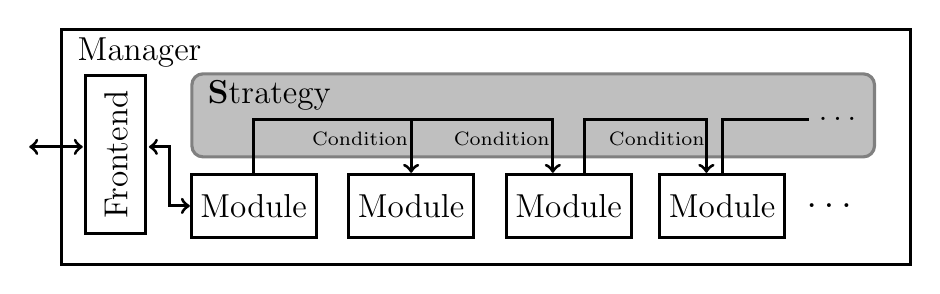
\begin{tikzpicture}[every node/.style={rectangle}, text centered, bend angle=15, line width=.4mm]
	\node[draw, minimum height=57pt, text width=15pt] (manager) at (-6.3, .2) {};
	\node[rotate=90] (managerText) at (-6.3, .2) {\large Frontend};
	\node[draw, minimum height=85pt, text width=300pt] (manager) at (-1.6, 0.3) {};
	\node[] (managerText) at (-6, 1.5) {\large Manager};
	\node[fill=lightgray,draw=gray, rounded corners, minimum height=30pt, text width=240pt] (strategy) at (-1,.7) {};
	\node[] (strategyText) at (-4.35, .95) {\large\textbf Strategy};
	\draw[<->] (-5.36,-.45) -- (-5.62,-.45) -- (-5.62,.3) -- (-5.88,.3);
	\draw[<->] (-6.72,.3) -- (-7.4,.3);
	\draw[->] (-4.55,-.03) -- (-4.55,.65) -- (-.75,.65) -- (-.75,-.03);
	\node[] (strategyText) at (-1.4, .4) {\scriptsize Condition};
	\draw[->] (-2.55,.65) -- (-2.55,-.03);
	\node[] (strategyText) at (-3.2, .4) {\scriptsize Condition};
	\draw[->] (-.35,-.03) -- (-0.35,.65) -- (1.2,.65) -- (1.2,-.03);
	\node[] (strategyText) at (.57, .4) {\scriptsize Condition};
	\draw (1.4,-.03) -- (1.4,.65) -- (2.5,.65);
	\node[] (dotsa) at (2.9,.65) {\large \ldots};
	\node[draw, minimum height=23pt] (moduleAText) at (-4.55, -.45) {\large Module};
	\node[draw, minimum height=23pt] (moduleBText) at (-2.55, -.45) {\large Module};
	\node[draw, minimum height=23pt] (moduleCText) at (-.55, -.45) {\large Module};
	\node[draw, minimum height=23pt] (moduleDText) at (1.4, -.45) {\large Module};
	\node[] (dotsc) at (2.8, -.45) {\Large \ldots};
\end{tikzpicture}%

\end{center}
\label{fig:frameworka}
\end{figure}

\begin{figure}[ht]
\caption{A snapshot of an \smtrat composition being a theory solver embedded in an SMT solver.}
\begin{center}
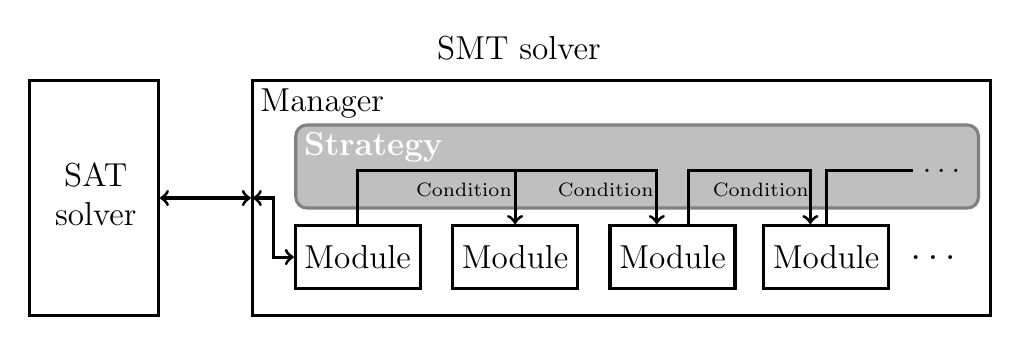
\begin{tikzpicture}[every node/.style={rectangle}, text centered, bend angle=15, scale=1, line width=.4mm]
	\node[] (smtsolver) at (-2.5, 2.2) {\large SMT solver};
	\node[draw, minimum height=85pt, text width=40pt] (satsolver) at (-7.9, 0.3) {\large\begin{tabular}{c}SAT \\ solver\end{tabular}};
	\node[draw, minimum height=85pt, text width=260pt] (manager) at (-1.2, 0.3) {};
	\node[] (managerText) at (-5, 1.5) {\large Manager};
	\node[fill=lightgray,draw=gray, rounded corners, minimum height=30pt, text width=240pt] (strategy) at (-1,.7) {};
	\node[] (strategyText) at (-4.35, .95) {\large\bf \color{white} Strategy};
	\draw[<->] (-5.36,-.45) -- (-5.62,-.45) -- (-5.62,.3) -- (-5.88,.3);
	\draw[->] (-4.55,-.03) -- (-4.55,.65) -- (-.75,.65) -- (-.75,-.03);
	\node[] (strategyText) at (-1.4, .4) {\scriptsize Condition};
	\draw[->] (-2.55,.65) -- (-2.55,-.03);
	\node[] (strategyText) at (-3.2, .4) {\scriptsize Condition};
	\draw[->] (-.35,-.03) -- (-0.35,.65) -- (1.2,.65) -- (1.2,-.03);
	\node[] (strategyText) at (.57, .4) {\scriptsize Condition};
	\draw (1.4,-.03) -- (1.4,.65) -- (2.5,.65);
	\node[] (dotsa) at (2.9,.65) {\large \ldots};
	\node[draw, minimum height=23pt] (moduleAText) at (-4.55, -.45) {\large Module};
	\node[draw, minimum height=23pt] (moduleBText) at (-2.55, -.45) {\large Module};
	\node[draw, minimum height=23pt] (moduleCText) at (-.55, -.45) {\large Module};
	\node[draw, minimum height=23pt] (moduleDText) at (1.4, -.45) {\large Module};
	\node[] (dotsc) at (2.8, -.45) {\Large \ldots};
	\path[<->] (satsolver.0) edge[] node[left] {} (manager.180);
\end{tikzpicture}

\end{center}
\label{fig:frameworkb}
\end{figure}

Based on \carl's data structures and basic functions, a rich set of SMT compliant implementations of \supportedLogics procedures is provided by \smtrat. Each procedure is encapsulated in a \emph{module}, which fixes a common interface, and they can then be composed to a solver according to a user defined \emph{strategy}. A \emph{manager} maintains their allocation to \emph{solving tasks} according to the strategy and provides the API, including the parsing of an \smtlibfile.

\section{Modules}
A module $m$ holds a set of formulas, called its \emph{set of received formulas} and denoted by $\Crcv(m)$. The main function of a module is \texttt{check(bool full)}, which either decides whether $\Crcv(m)$ is satisfiable or not, returning \SAT or \UNSAT, respectively, or returns \UNKNOWN. A set of formulas is semantically defined by their conjunction. If the function's argument \texttt{full} is set to \false, the underlying procedure of $m$ is allowed to omit hard obstacles during solving at the cost of returning \UNKNOWN in more cases. We can manipulate $\Crcv(m)$ by adding (removing) formulas $\varphi$ to (from) it with \texttt{add($\varphi$)} (\texttt{remove($\varphi$)}). Usually, $\Crcv(m)$ is only slightly changed between two consecutive \texttt{check} calls, hence, the solver's performance can be significantly improved if a module works incrementally and supports backtracking. In case $m$ determines the unsatisfiability of $\Crcv(m)$, it has to compute at least one preferably small \emph{infeasible subset} $\Cinf(m)\subseteq \Crcv(m)$. Moreover, a module can specify \emph{lemmas}, which are valid formulas. They encapsulate information which can be extracted from a module's internal state and propagated among other modules. Furthermore, a module itself can ask other modules for the satisfiability of its \emph{set of passed formulas} denoted by $\Cpass(m)$, if it invokes the procedure \texttt{runBackends(bool full)} (controlled by the manager). It thereby delegates work to modules that	 may be more suitable for the problem at hand. 

\section{Strategy}
\label{sec::strategy}
\smtrat allows a user to decide how to compose the modules. For this purpose we provide a graphical user interface, where the user can create a \emph{strategy} specifying this composition. A strategy is a directed tree $T:=(V, E)$ with a set $V$ of modules as nodes and $E\subseteq V\times \Omega\times\Sigma\times V$, with $\Omega$ being the set of \emph{conditions} and $\Sigma$ being the set of \emph{priority values}. A condition is an arbitrary Boolean combination of formula properties, such as propositions about the Boolean structure of the formula, e.g., whether it is in conjunctive normal form (CNF), about the constraints, \eg whether it contains equations, or about the polynomials, e.g., whether they are linear. Furthermore, each edge carries a unique priority value from $\Sigma=\{1,\ \ldots,\ |E|\}$.

\section{Manager}
The \emph{manager} holds the strategy and the SMT solver's input formula $C_{input}$. Initially, the manager calls the method \texttt{check} of the module $m_r$ given by the root of the strategy with $\Crcv(m_r) = C_{input}$. Whenever a module $m\in V$ calls \texttt{runBackends}% for its passed formula $\Cpass(m)$
, the manager adds a \emph{solving task} $(\sigma,\ m,\ m')$ to its priority queue $Q$ of solving tasks (ordered by the priority value), if there exists an edge $(m,\ \omega,\ \sigma,\ m')\in E$  in the strategy such that $\omega$ holds for $\Cpass(m)$. If a processor $p$ on the machine where \smtrat is executed on is available, the first solving task of $Q$ is assigned to $p$ and popped from $Q$. The manager thereby starts the method \texttt{check} of $m'$ with $\Crcv(m') = \Cpass(m)$ and passes the result (including infeasible subsets and lemmas) back to $m$. The module $m$ can now benefit in its solving and reasoning process from this shared information. Note that a strategy-based composition of modules works incrementally and supports backtracking not just within one module but as a whole. This is realized by a mapping in each module $m$ of its passed formulas $\varphi\in\Cpass(m)$ to sets $R_1,\ldots,\ R_n \subseteq \Crcv(m)$ such that each $R_i$ forms a reason why $m$ included $\varphi$ in $\Cpass(m)$ to ask for its satisfiability. In order to exploit the incrementality of the modules, all parallel executed backends terminate in a consistent state (instead of just being killed), if one of them finds an answer.
  
\section{Procedures implemented as modules}
\label{sec:implemented_modules}
The heart of an SMT solver usually forms a SAT solver. In \smtrat, the module \satModule abstracts $\Crcv(\satModule)$ to propositional logic and uses the efficient SAT solver \texttt{minisat}~\cite{minisat} to find a Boolean assignment of the abstraction. It invokes \texttt{runBackends} where $\Cpass(\satModule)$ contains the constraints abstracted by the assigned Boolean variables in a less-lazy fashion~\cite{sebastiani2007lazy}. The module \simplexModule implements the Simplex method equipped with branch-and-bound and cutting-plane procedures as presented in \cite{DM06}. We apply it on the linear constraints of any conjunction of \supportedLogics constraints. For a conjunction of nonlinear constraints \smtrat provides the modules \gbModule, \vsModule and \cadModule, implementing GB~\cite{JLCA_CAI13}, VS~\cite{Article_Corzilius_FCT2011} and CAD~\cite{Article_Loup_TubeCAD} procedures, respectively. Moreover, the module \icpModule uses ICP similar as presented in~\cite{GGIGSC10}, lifting splitting decisions and contraction lemmas to a preceding \satModule and harnessing other modules for nonlinear conjunctions of constraints as backends. The exact procedure is going to be published. The module \cnfModule invokes \texttt{runBackends} on $\Cpass(\cnfModule)$ being the CNF of $\Crcv(\cnfModule)$, and the module \ppModule performs some preprocessing based on factorizations and sum-of-square decompositions of polynomials.

\section{Infeasible subsets and lemmas}
\label{sec::infsubset_lemmas}
Infeasible subsets and lemmas, which contain only formulas from 
$\Cpass(\SATM)$, prune the Boolean search space and hence the number of theory calls. 
Smaller infeasible subsets are usually more advantageous, because they make larger cuts 
in the search space. Lemmas containing new constraints we call
\emph{inventive lemmas} (\emph{non-inventive} otherwise). They might enlarge the 
Boolean search space, but they can reduce the complexity of later theory calls.
When using inventive lemmas, it is important to ensure that the set possible
constraints introduced in such lemmas is finite for a given module and a given 
input formula. Otherwise, the termination of this procedure can not be guaranteed.



\chapter{Embedding of a theory solver into an SMT solver}
\label{chapter:embeddingats}
In the following we assume, that either a composed theory solver according
to Chapter~\ref{chapter:composingats} or the composition we provide, i.e.
the \texttt{NRATSolver}, is used. They only differ in the strategy they implement
and provide the same interfaces. We give a short description of these
interfaces and give an example by embedding it into \Opensmt.

\section{Interfaces of a theory solver composed with \smtrat}
An SMT solver can use the following interfaces:
\begin{itemize}
	\item \begin{verbatim}bool inform( const string& _constraint, bool _infix )\end{verbatim}
		Informs the theory solver about the existence of the given constraint in form of
		a string. The second argument is a flag, which indicates whether the given constraint
		is written in infix or prefix notation.
	\item \begin{verbatim}
		bool addConstraint
		(
		    const string& _constraint,
		    const bool _infix,
		    const bool _polarity
		)
		\end{verbatim}
		Adds the given constraint in form of a string to the theory solver. The second argument 
		is a flag, which indicates whether the given constraint is written in infix or prefix 
		notation. The last argument is again a flag which is \true if the constraint
		has to hold in the given form and \false if its inversion has to hold. The inversion 
		operator for a constraint simply changes its relation symbol in the following way:
		$$\begin{array}{ccc}
			= & \mapsto & \neq \\
			\neq & \mapsto & = \\
			\leq & \mapsto & > \\
			\geq & \mapsto & < \\
			< & \mapsto & \geq \\
			> & \mapsto & \leq \\
		\end{array}$$\\[2ex]
		
    \item \begin{verbatim}Answer isConsistent( )\end{verbatim}
    	Checks the so far received constraints for consistency. The answer can either be
    	\true, if the set of the so far received constraints is consistent, or 
    	\false, if it is inconsistent, and \texttt{unknown}, if the theory 
    	solver cannot reason about it.
    \item \begin{verbatim}void pushBacktrackPoint( )\end{verbatim}
    	Pushes a backtrack point to the stack of backtrack points.
    \item \begin{verbatim}void popBacktrackPoint( )\end{verbatim}
    	Pops a backtrack point from the stack of backtrack points and undoes everything
		which has been done after adding that backtrack point.
    \item \begin{verbatim}vector< vector< unsigned > > getReasons( )\end{verbatim}
    	Returns one or more reasons for the inconsistency of the constraints. A reason
    	is an infeasible subset of the so far received constraints. An element of a reason
    	is a number $i$ and means that the $i$th received constraint is an element of
    	this infeasible subset.
\end{itemize}

\section{Example: Embedding a \smtrat composition into \opensmt}
\opensmt is an open source SMT solver and supports the embedding of additional
theory solver. A detailed instruction of how to extend \opensmt by a theory solver
can be found on \opensmtURL. Unfortunately, \opensmt does not yet support
quantifier free nonlinear real arithmetic (QF\_NRA). For the following we assume 
that it supports QF\_NRA and create a theory solver using the interfaces
\opensmt provides.

\begin{figure}[htb] 
\begin{verbatim}
class TSolver 
{
    void   inform        ( Enode * ); 
    bool   assertLit     ( Enode * ); 
    bool   check         ( bool ); 

    void   pushBktPoint  ( ); 
    void   popBktPoint   ( ); 
    bool   belongsToT    ( Enode * ); 
    void   computeModel  ( ); 

    vector <  Enode *  >  & explanation; 
    vector <  Enode *  >  & deductions; 
    vector <  Enode *  >  & suggestions; 
}
\end{verbatim}
\end{figure}
\newpage
\noindent\opensmt gives the following explanation:

\begin{quote}
	"\texttt{inform} is used to communicate the existence of a new T-atom to the T-solver. 
	\texttt{assertLit} asserts a (previously informed) T-atom in the T-solver with the right 
	polarity; it may also perform some cheap form of consistency check. 
	\texttt{check} determines the T-satisfiability of the current set of asserted T-atoms. 
	\texttt{pushBktPoint} and \texttt{popBktPoint} are used respectively to save and to restore 
	the state of the T-solver, in order to cope with backtracking within the 
	SAT-Solver. \texttt{belongsToT} is used to determine if a given T-atom belongs to 
	the theory solved by the T-solver. Finally \texttt{computeModel} forces T-solver to 
	save the model (if any) inside Enode's field.

	Three vectors, \texttt{explanation}, \texttt{deductions}, \texttt{suggestions}, are 
	shared among the T-solvers, and they are used to simplify the communication of conflicts, 
	T-atoms to be deduced and "suggested" T-atoms. Suggestions are atoms 
	consistent with the current state of the T-solver, but that they cannot be 
	directly deduced. Suggestions are used to perform decisions in the 
	SAT-Solver."~\footnote{http://verify.inf.usi.ch/opensmt/build-your-solver}
\end{quote}
\noindent We derive a theory solver and extend it by the three additional members
\begin{itemize}
	\item \texttt{mpManager}, being a pointer to the theory solver object, 
	\item \texttt{mReceivedEnodes}, needed to reconstruct which enode corresponds
		to which constraint,
	\item \texttt{mBackendsBacktrackpoints}, to store the backtrack points.
\end{itemize}
Figure~\ref{fig:headernrasolver} shows the resulting code for the header of the theory 
solver within \opensmt. The constructor of the embedded	theory solver is shown in 
Figure~\ref{fig:constructornrasolver}. Note, that instead of \texttt{NRATSolver} any other 
\smtrat-composition can be used. Figure~\ref{fig:informnrasolver}
shows the method which informs the theory solver about the existence of a constraint.
Here, we first get the string representation of the constraint, which is in prefix notation,
and pass it to the \texttt{NRATSolver}. Note, that, for a reason
we are not aware of, the return value has to be \texttt{lbool} and not, as mentioned on 
the webpage, \texttt{void}. The method \texttt{assertLit}, 
given by Figure~\ref{fig:assertLitnrasolver}, takes again the string representation of the given
literal/constraint and adds it to the \texttt{NRATSolver}. The return value is \false
if the constraint is inconsistent and \true otherwise. Note, that the polarity indicates
whether the literal is positive or negative. A negativ fulfilled literal implies that
the aforementioned inversion of the constraint has to hold. The implementation of the 
method \texttt{pushBacktrackPoint} shown by Figure~\ref{fig:pushBacktrackPointnrasolver}
is straightforward. 

Figure~\ref{fig:popBacktrackPointnrasolver} shows the implementation
of the method \texttt{popBacktrackPoint}. It first empties the explanation vector and then
removes all stored enodes, which have been added after the backtrack point to remove.
Finally, it pops the backtrack point within the theory solver used by \opensmt and
calls \texttt{popBacktrackPoint} of the \texttt{NRATSolver}. The check procedure
given in Figure~\ref{fig:checknrasolver} calls \texttt{isConsistent} of
the \texttt{NRATSolver}. The easiest case is if the return value is \true.
Then we know that the set of the so far added constraints is consistent and return
\true. If it determines inconsistency, that is \texttt{isConsistent} returns
\false, we extract one reason for the inconsistency and store the 
corresponding literals in the explanation vector. This is why we need to store
the so far received literals. Finally, we return \false. Note, that we might obtain 
more than one reason. However, \opensmt does not support more than one reason and 
we discard the other reasons. The case of getting the answer \texttt{unknown} is 
unfortunately not supported by \opensmt.


\begin{figure}[htb]
\caption{The header implementation of a theory solver used by \opensmt.}
\label{fig:headernrasolver}
\begin{verbatim}
#include "TSolver.h"
#include <smt-rat/smt-rat.h>

class NRASolver : public OrdinaryTSolver
{
public:
    NRASolver( const int           
          	, const char *        
      	    , SMTConfig &         
      	    , Egraph &            
      	    , SStore &
      	    , vector< Enode * > & 
      	    , vector< Enode * > & 
          	, vector< Enode * > & );

  	~NRASolver ( );

  	lbool   inform              ( Enode * );               
  	bool    assertLit           ( Enode *, bool = false ); 
  	void    pushBacktrackPoint  ( );                       
  	void    popBacktrackPoint   ( );                       
  	bool    check               ( bool );                  
  	bool    belongsToT          ( Enode * );               
  	void    computeModel        ( );                       
#ifdef PRODUCE_PROOF
  	Enode * getInterpolants     ( );
#endif

private:
    Manager*         mpManager     ;
    vector< Enode* >   mReceivedEnodes ;
    vector< unsigned > mBacktrackPoints;
};
\end{verbatim}
\end{figure}

\begin{figure}[htb]
\caption{The constructor of a theory solver used by \opensmt.}
\label{fig:constructornrasolver}
\begin{verbatim}
NRASolver::NRASolver( const int           i
                    , const char *        n
                    , SMTConfig &         c
                    , Egraph &            e
                    , SStore &            t
                    , vector< Enode * > & x
                    , vector< Enode * > & d
                    , vector< Enode * > & s )
             : OrdinaryTSolver ( i, n, c, e, t, x, d, s )
{
    mpManager      = new NRATSolver()    ; \\ This could also be
                                           \\ your theory solver
                                           \\ composition.
    mReceivedEnodes	 = vector< Enode* >()  ;
    mBacktrackPoints = vector< unsigned >();
}
\end{verbatim}
\end{figure}


\begin{figure}[htb]
\caption{The method to inform the theory solver used by \opensmt about a constraint.}
\label{fig:informnrasolver}
\begin{verbatim}
lbool NRASolver::inform(Enode *e)
{
    (void)e;
    assert(e);
    assert(belongsToT(e));

    ostringstream stream;
    stream << e;

    mpManager->inform( stream.str(), false );

    return l_Undef;
}
\end{verbatim}
\end{figure}

\begin{figure}[htb]
\caption{The method to assert a literal in a theory solver used by \opensmt.}
\label{fig:assertLitnrasolver}
\begin{verbatim}
bool NRASolver::assertLit( Enode *e, bool reason )
{
    (void)e;
    (void)reason;
    assert(e);
    assert(belongsToT(e));

    mReceivedEnodes.push_back( e );

    ostringstream stream;
    stream << e;

    return mpManager->addConstraint( stream.str()            , 
                                     false                   , 
                                     e->getPolarity()==l_True );
}
\end{verbatim}
\end{figure}

\begin{figure}[htb]
\caption{The method to push a backtrack point in a theory solver used by \opensmt.}
\label{fig:pushBacktrackPointnrasolver}
\begin{verbatim}
void NRASolver::pushBacktrackPoint()
{
    mBacktrackPoints.push_back( mReceivedEnodes.size() );
    mpManager->pushBacktrackPoint();
}
\end{verbatim}
\end{figure}

\begin{figure}[htb]
\caption{The method to pop a backtrack point in a theory solver used by \opensmt.}
\label{fig:popBacktrackPointnrasolver}
\begin{verbatim}
void NRASolver::popBacktrackPoint( )
{
    explanation.clear();

    while( mBacktrackPoints.back()<mReceivedEnodes.size() )
    {
        mReceivedEnodes.pop_back();
    }

    mBacktrackPoints.pop_back();

    mpManager->popBacktrackPoint();
}
\end{verbatim}
\end{figure}

\begin{figure}[htb]
\caption{The method to check for consistency in a theory solver used by \opensmt.}
\label{fig:checknrasolver}
\begin{verbatim}
bool NRASolver::check( bool _complete )
{
    (void)_complete;

    switch( mpManager->isConsistent() )
    {
        case TS_True: return true;
        case TS_False:
        {
            vector< vector< unsigned > > reasons
                = mpManager->getReasons();
            vector< unsigned >::const_iterator pos
                = reasons.back().begin();
            while( pos!=reasons.back().end() )
            {
                explanation.push_back( mReceivedEnodes.at( *pos ) );
                ++pos;
            }
      	    return false;
        }
        case TS_Unknown: assert( false );
        default: assert( false );
    }
}
\end{verbatim}
\end{figure}



\chapter{Implementing further modules}
\label{chapter:implementingamodule}
In this chapter we explain how to implement further modules. A module is a derivation
of the class \texttt{Module} and we give an 
introduction to its members, interfaces and auxiliary methods in the following of this
chapter. A new module and, hence, the corresponding \Cpp source and header files can be easily
created when using the script \texttt{writeModules.py}. Its single argument is the module's name
and the script creates a new folder in \texttt{src/lib/modules/} containing the
source and header file with the interfaces yet to implement. A new module should be created
only this way, as the script takes care of a correct integration of the corresponding code
into \smtrat.

\section{Members of a module}
Here is an overview of those members of the class \texttt{Module}, which can be accessed directly.
They form the most important ones for an implementation of a new module.

\begin{itemize}
	\item \begin{verbatim}vector<set<const Formula*>> mInfeasibleSubsets\end{verbatim}
		Stores the infeasible subsets of the so far received formulas, if the module determined that
		their conjunction is not satisfiable.
	\item \begin{verbatim}Manager* const mpManager\end{verbatim}
		A pointer to the manager which maintains the allocation of modules (including this one) to other 
		modules, when they call a backend for a certain formula. For further details see Chapter~\ref{chapter:composingats}.
	\item \begin{verbatim}Formula* mpReceivedFormula\end{verbatim}
		Stores the conjunction of the so far received formulas, which this module considers
		for a satisfiability check.
	\item \begin{verbatim}Formula* mpPassedFormula\end{verbatim}
		Stores the conjunction of the formulas which this module has passed to a backend to be
		solved for satisfiability.
\end{itemize}

\section{Interfaces to implement}
In the following we explain which interfaces must be implemented in a module.

\subsection{Informing about a constraint}
\begin{figure}[htb]
\label{fig:exa_inform}
\caption{Example showing how to implement the method \texttt{inform}}
\begin{verbatim}
	bool MyModule::inform( const Constraint* const  _constraint )
	{
	    // Write the implementation here.
	}
\end{verbatim}
\end{figure}
Informs the module about the existence of the given constraint usually before
any formula containing constraints is added to this module for consideration
of a later satisfiability check. At least it can be expected, that this method
is called, before a formula containing the given constraint is added 
to this module for consideration of a later satisfiability check. 
Note that this information might be useful for the module, e.g., for the 
initialization of the datastructures it uses.

\subsection{Asserting a received formula}
\begin{figure}[htb]
\label{fig:exa_assertsubformula}
\caption{Example showing how to implement the method \texttt{assertSubformula}}
\begin{verbatim}
	bool MyModule::assertSubformula( Formula::const_iterator _subformula )
	{
	    Module::assertSubformula( _subformula );
	    // Write the implementation here.
	}
\end{verbatim}
\end{figure}
Asserts the formula at the given position in the conjunction of received formulas 
(\texttt{mpReceivedFormula}), meaning that this module has to include this formula
in the next satisfiability check. If the module
can already decide whether the given formula is not satisfiable itself, it returns \false
otherwise \true. In comparison to the interface \texttt{inform}, any previous solving results
could be consulted to determine this information.
Note, that the implementation of a new module might need some initialization in this method
and has always to call \texttt{Module::assertSubformula} at the beginning.

\subsection{Removing a received formula}
\begin{figure}[htb]
\label{fig:exa_removesubformula}
\caption{Example showing how to implement the method \texttt{removeSubformula}}
\begin{verbatim}
	void MyModule::removeSubformula( Formula::iterator _subformula )
	{
	    // Write the implementation here.
	    Module::removeSubformula( _subformula );
	}
\end{verbatim}
\end{figure}
Removes the formula at the given position from the conjunction of received formulas
(\texttt{mpReceivedFormula}). Everything,
which has been stored in this module and depends on this formula must be removed. In the end of
this method, \texttt{Module::removeSubformula} must be called. It handles the removing of everything
depending on this formula in the derived members of this module, including the infeasible subsets,
the passed formula and the mapping of passed formulas to received formulas, which is introduced in
Section~\ref{sec:runbackend}. Hence, you do not need to take care of this.

\subsection{Checking for satisfiability}
\begin{figure}[htb]
\label{fig:exa_check}
\caption{Example showing how to implement the method \texttt{check}}
\begin{verbatim}
	Answer MyModule::check()
	{
	    // Write the implementation here.
	}
\end{verbatim}
\end{figure}
Implements the actual satisfiability check of the conjunction of formulas, which have been asserted in this module.
There are three options how this module can answer: it either determines that the formulas
are satisfiable and returns \true, it determines unsatisfiability and returns
\false, or it cannot give a conclusive answer and returns \texttt{unknown}. Note, that the method \texttt{Answer foundAnswer( Answer )} must
be invoked with the found answer, before return it. Its return value has the same value as its argument and, hence, you could call it the
following (prettying) way:
\begin{verbatim}
Answer MyModule::check()
{
    ...
    return foundAnswer( yourAnswer );
}
\end{verbatim}
Furthermore, modules can always call
a backend in order to check the satisfiability of any conjunction of formulas. How to run the backend is shown in
Section~\ref{sec:runbackend}. A module has also the opportunity to reason about the conflicts
occurred, if it determines unsatisfiability. For this purpose it has store at least one infeasible
subsets of the set of so far received formulas.

\section{Running backend modules}
\label{sec:runbackend}
Modules can always call a backend in order to check the satisfiability of any conjunction of formulas.
Fortunately, there is no need to manage the assertion or removement of formulas to the backend. 
This would be even more involved as we do allow changing the
backend if it is appropiate (more details to this are explained in Chapter~\ref{chapter:composingats}).
Running the backend is done in two steps:
\begin{enumerate}
	\item Change the passed formula to the formula which should be solved by the backend. Keep in mind,
	       that the passed formula could still contain formulas of the previous backend call.
	\item Call \texttt{runBackends()}.
\end{enumerate}
The first step is a bit more tricky, as we need to know which received formulas led to a passed
formula. For this purpose a module contains a mapping from a passed formula to one or more
sets of received formulas. We give a small example by showing the behavior of one of the modules
we provide, the \simplifierModuleClass. Let us assume that this module has so far received the following
constraints:
$$c_0:x\leq0,\ c_1:x\geq 0,\ c_2:x=0$$
\simplifierModuleClass combines the first two constraints $c_0$ and $c_1$ to $c_3:x=0$. Then it combines
$c_3$ with $c_2$ to $c_5:x=0$. Afterwards it calls its backend on the only remaining constraint,
that means the passed constraints contain only $c_5:x=0$. The mapping of $c_5$ to the received constraints it
stems from is $$c_5\ \mapsto\ (\{c_0,\ c_1\},\ \{c_2\}).$$

The mapping is maintained automatically and offers two methods to add formulas to the vector
of the passed formulas:
\begin{itemize}
	\item \begin{verbatim}void addReceivedSubformulaToPassedFormula( Formula::const_iterator )\end{verbatim}
		Adds the formula at the given positition in the conjuntion of the so far received formulas
		to the conjunction of the passed formulas. The mapping to its \emph{original formulas} contains
		only the formula at the given position in the vector of received formula
	\item
		\begin{verbatim}
		void addSubformulaToPassedFormula
		(
		    Formula*,
		    const vec_set_const_pFormula&
		)
		\end{verbatim}
		Adds the given formula to the vector of the passed formulas. It is mapped to the given
		original formulas. Note, that the second argument must contain only subformulas of the conjunction 
		of so far received formulas. We	do not check this by reason of efficiency.
\end{itemize}
If the original formulas of a passed formula are only empty sets, by reason of a belated removing of the according
received formulas, this passed formula will be automatically removed from the backends and the passed formula.

The second step is really just calling \texttt{runBackends()} and processing its return value, which can be
\true, \false, or \texttt{unknown}.

\section{Auxilliary functions}
The \texttt{module} class provides a rich set of methods for debugging purposes. Besides some 
printing methods, \smtrat helps to maintain the correctness of new modules during their development.
It therefore provides methods to store formulas with their assumed satisfiability status in order
to check them belatedly by any SMT solver which is capable to parse \texttt{.smt2} files and solve
the stored formula. To be able to use the following methods, the compiler flag \texttt{SMTRAT\_DEVOPTION\_Validation}
must be activated, which can be easily achieved when using \ccmake.

\begin{itemize}
	\item \begin{verbatim}static void addAssumptionToCheck( const X&, bool, const string& ) \end{verbatim}
		Adds the given formulas to those, which are going to be stored as an \texttt{.smt2} file,
		with the assumption that they are satisfiable, if the given Boolean argument is \true, or unsatisfiable,
		if the given Boolean argument is \false. The formulas can be passed as one of the following types (\texttt{X} can be one of the following datastructures)
		\begin{itemize}
		\item \texttt{Formula} (a single formula of any type)
		\item \texttt{set<const Formula*>} (a set of formulas, which is considered to be a conjunction)
		\item \texttt{set<const Constraint*>} (a set of constraints, which is considered to be a conjunction)
		\end{itemize}
		The third argument of this function is any string which helps to identify the assumption, e.g.,
		involving the name of the module and for which purpose this assumption has been made.
	\item \begin{verbatim}static void storeAssumptionsToCheck( const Manager& )\end{verbatim}
		This method stores all collected assumptions to the file \texttt{assumptions.smt2}, which can be checked
		later by any SMT solver which is capable to parse \texttt{.smt2} files and solve
		the stored formula. As this method is static, we need to pass the module's manager (\texttt{*mpManager}).
		Note that this method will be automatically called when destructing the given manager. Invoking this
		method is only reasonable, if the solving aborts directly afterwards and, hence, omits the manager's
		destructor.
	\item \begin{verbatim}void checkInfSubsetForMinimality
(
    vector<set<const Formula*>>::const_iterator,
    const string&,
    unsigned
) const 
\end{verbatim}
This method checks the infeasible subset at the given position for minimality, that is it checks whether there is a subset of it having maximally $n$ elements less, which is still infeasible.
As for some approaches it is computationally to hard to provide always a minimal infeasible subset, they rather provide infeasible subsets not necessarily being minimal. This method helps 
to ananlyze how close the size of the encountered infeasible subsets is to a minimal one.
\end{itemize}



\chapter{Composing a solver}
\label{chapter:composingats}
\smtrat contributes a toolbox for composing an SMT compliant solver for real arithmetic, that means it 
is incremental, supports backtracking and provides reasons for inconsistency. The resulting
solver is either a fully operative SMT solver for real arithmetic, which can be applied
directly on \texttt{.smt2}-files, or a theory solver, which can be embedded into an SMT 
solver in order to extend its supported logics by real arithmetic.

We are talking about composition and toolbox, as \smtrat contains implementations
of many different mathematical approaches to tackle real arithmetic, each of them
embedded in a module with uniform interfaces. Theses modules form the tools in the toolbox
and it is dedicated to a user how we use them for solving a real arithmetic formula.
We provide a self-explanatory graphical user interface (GUI) for defining a graph-based 
strategy specifying which module(s) should be applied on which formula, 
taking into account the modules we have already involved.

In Section~\ref{sec:managerstrategy} we have already introduced
a strategy and in the following of this chapter we firstly give a brief introduction 
to the existing modules equipped with an estimation of their input-based performances and then illustrate
how to use the GUI for composing a strategy.

\section{Existing module implementation}
\subsection{The \texttt{CNFerModule}}
\subsection{The \texttt{PreprocessingModule}}
\subsection{The \texttt{SATModule}}
\subsection{The \texttt{LRAModule}}
\subsection{The \texttt{GBModule}}
\subsection{The \texttt{VSModule}}
\subsection{The \texttt{CADModule}}

\section{Specifying a strategy with the GUI}

The presented GUI is called SMT-XRAT. The GUI possesses an own name to highlight, that it is a standalone program apart of the actual toolbox. The name simply derives from SMT-RAT and adds the letter `X' to symbolize, that it is a graphical window application, whereas the toolbox is operated in the console.

The following subsections are used to give an overview of SMT-XRAT and to introduce its functionalities. Besides the required features, additional features are stated, which have been implemented to gain a higher degree of usability and user experience. These features help to prevent user frustrations, enable fail-safe working and support the visual creation and manipulation process of strategy graphs.

\subsection{Concept}
\label{sec:concept_of_smt-xrat}
The underlying concept of SMT-XRAT is the user-guided, visual modeling of module compositions in form of graphs and their mapping onto their corresponding source code for SMT-RAT. A modeled graph expresses an intended strategy graph of the user. Both can easily be projected on each other, because the data structure of a strategy graph also describes a graph structure, as explained in the previous chapter. A mapping considers not only the modeled hierarchy of the SMT-RAT modules, but also their attributes. Furthermore the GUI complies the constraints of these attributes during the modeling process, for example priority values are required to be unique.

The user benefits from that concept, because strategy graphs can be created and manipulated completely independent of SMT-RAT. No knowledge of the inner data structure of strategy graphs and no knowledge about their corresponding source code is required by the user. The GUI does not only support the visual creation of strategy graphs and their translation into source code, but also enables the user to integrate the translated source code into SMT-RAT or, if necessary, delete it subsequently. The conclusive work only involves a recompilation of SMT-RAT with the desired strategy graph instance to obtain a customized SMT solver.

SMT-XRAT has been implemented with the programming language Java. It embeds the freely available Java Universal Network/Graph Framework (JUNG) \cite{JUNG}, which fulfills the main demands of the underlying concept, as it allows to model and visualize data, which can be represented as a graph. The JUNG library helped to reduce the basic workload of the GUI creation enormously. Even though, a lot of effort still remained in adjusting its classes to fit for SMT-XRAT.

\subsection{Main window structure}
\label{sec:main_window_structure_of_smt-xrat}
The main window structure of the SMT-XRAT application can be seen in Figure \ref{fig:smt-xrat_main_window}. It principally consists only of one large pane, which is called \emph{strategy graph pane}. This pane embodies the workspace of the user and visualizes the composition of SMT-RAT modules, which are currently modeled. Only a comparatively small area is occupied by a compact menu bar, which offers further necessary or practical functionalities, but which need no visualizations, for instance the exportation of a strategy graph into SMT-RAT.
\begin{figure}
  \begin{center}
    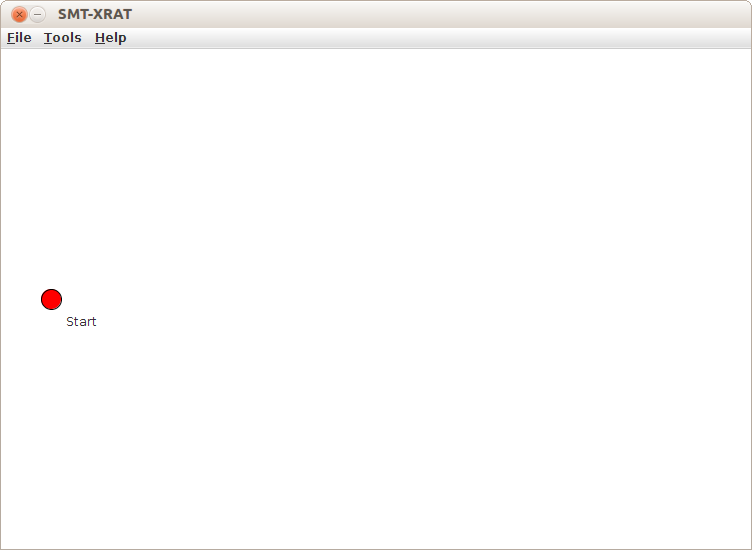
\includegraphics[width=0.9\textwidth]{graphics/smt-xrat_main_window.png}
  \end{center}
  \caption{The main window of the SMT-XRAT application in its initial state.}
  \label{fig:smt-xrat_main_window}
\end{figure}

\subsection{Strategy graph pane}
\label{sec:the_strategy_graph_pane}
The strategy graph pane is the focus point of the main window and occupies nearly all of its area. It can hereby offer enough workspace to the user to model strategy graphs without distractions. Modeled graphs are acyclic, directed and weakly connected, right as they are needed for Grammar ${\cal SG}$. Nodes represent SMT-RAT modules and edges represent the call hierarchy of them. Both of the element types are labeled to display all necessary and editable module attributes within the visualization. Thereby the user is always able to keep a full overview of the modeled strategy graph and its attributes. Moreover, the user can continuously be aware of the presented execution flow of the module composition. Thus, SMT-XRAT nicely supports the user to visualize an imagined strategy while mapping it onto a data structure in the same time.

Modeling strategy graphs on the pane implies the interactive operations of adding, editing and deleting modules and also aligning elements, if desired by the user.

\subsubsection{Adding backends}
\label{sec:adding_backends}
\begin{figure}
  \begin{center}
    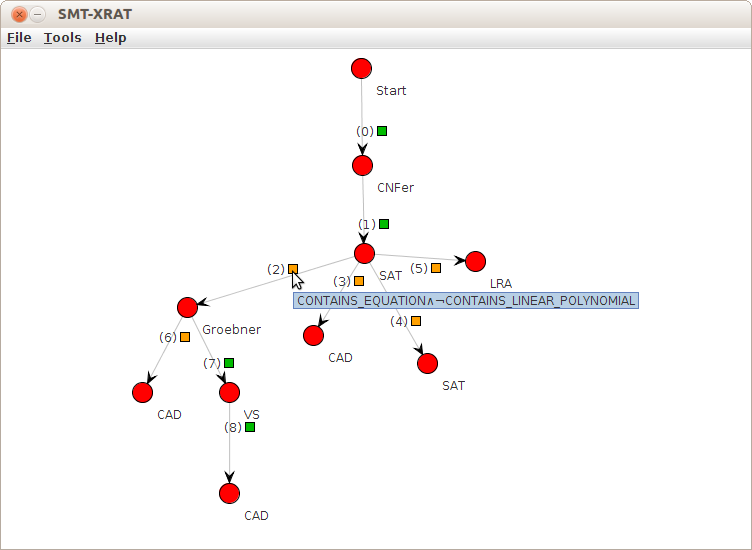
\includegraphics[width=0.9\textwidth]{graphics/smt-xrat_condition_ttt.png}
  \end{center}
  \caption{The small rectangles alongside the edges reveal the hidden condition of a backend.}
  \label{fig:smt-xrat_condition_ttt}
\end{figure}

An initial visualization of the pane contains the inevitable \emph{Start} module of an SMT solver, which displays no attributes, but marks the starting point for the user to create the desired strategy graph. The user can simply consider the \emph{Start} module as the frontend of an SMT solver where NRA problems are passed to. Building up a composition of modules occurs by appending backends to the \emph{Start} module and then to the newly appended backends and so forth. When appending a backend to a selected module, a dialog window requests the operating user to input a condition and to choose the type of SMT-RAT module for the new backend. The GUI provides a special input interface to enter conditions, which is explained later. For each appended backend a new node as well as a directed edge from the originating module to this new node is drawn in the visualization. In this way, the graph gradually arises on the pane. The added graph elements display the inputted data of a backend. A node is labeled with 
its 
type of SMT-RAT module whereas an edge holds its condition and an automatically assigned priority value. Initially this priority value is always the total number of currently existing modules decreased by 1, as the \emph{Start} module is not counted. As inputted conditions might get quite long, they cannot be directly seen on the strategy graph pane. Instead, a small rectangle alongside the edge reveals them quickly on request. The user needs to point the mouse cursor over a rectangle to obtain its corresponding tool tip text, which shows the hidden condition, as can be seen in Figure \ref{fig:smt-xrat_condition_ttt}. This leaves the graph compact and helps to concentrate on the more essential aspect of modeling an execution hierarchy. The user can choose to input an own condition or leave it by the default value of `\texttt{TRUE}', which, as described in the last 
chapter, means that a condition is always satisfied. To point out better which modules contain default conditions and which do not, the color of a rectangle containing a default condition is green and otherwise orange. When looking at the strategy graph pane, the user is always capable to recognize the execution flow of the modules by following the directed edges in the graph. The colored rectangles signalize at which points of the hierarchy a passed formula must be checked against the condition for an intended backend. This is a quite handy feature, when the user wants to re-enact the solving of an SMT problem.

\subsubsection{Grammar for conditions}
\label{sec:grammar_for_backend_conditions}
When adding a module to the strategy graph pane, the user has to input a valid condition for its intended use as backend. A valid condition is a derivation of the formal Grammar $\cal C$, which completes Grammar $\cal SG$ of Definition \ref{def:grammar_strategy_graph} of the previous chapter. The grammar is concretely utilized by the GUI. A recursive descent parser \cite{ALSU07} has been implemented in the GUI, which applies exactly this grammar.
Conditions are derived from the formal Grammar $${\cal C}=(N, \Sigma, R, S).$$ The set of nonterminals is given by $$N=\{S, T, B, C, D, P\},$$ whereas the set of terminal symbols $$\Sigma=\{\texttt{(}, \texttt{)}, \neg, \leftrightarrow, \oplus, \rightarrow, \land, \lor\} \cup \{\texttt{TRUE}, \texttt{p}_1, \dots, \texttt{p}_n \}$$ consists of the union of logical operators and propositions. $S \in N$ is the start symbol of the production rules denoted by the set $R$, which covers the following:
\begin{center}
\begin{tabular}{lccccccccccc}
  $S$ & $\rightarrow$ & \texttt{TRUE} & $|$ & $T$ & $|$ & $C$ & $|$ & $D$ & $|$ & $TBT$ \\
  $T$ & $\rightarrow$ & $P$ & $|$ & $\neg T$ & $|$ & \texttt{(}$C$\texttt{)} & $|$ & \texttt{(}$D$\texttt{)} & $|$ & \texttt{(}$TBT$\texttt{)} \\
  $B$ & $\rightarrow$ & $\leftrightarrow$ & $|$ & $\oplus$ & $|$ & $\rightarrow$ \\
  $C$ & $\rightarrow$ & $C\land C$ & $|$ & $T$ \\
  $D$ & $\rightarrow$ & $D\lor D$ & $|$ & $T$ \\
  $P$ & $\rightarrow$ & $\texttt{p}_1$ & $|$ & \dots & $|$ & $\texttt{p}_n$ \\
\end{tabular}
\end{center}

The nonterminal symbols stay for the following: As said, $S$ for the start symbol of the production rules, $T$ for term, $B$ for binary operator, $C$ for conjunction, $D$ for disjunction and $P$ for proposition.

The terminals `$\neg$', `$\leftrightarrow$', `$\oplus$', `$\rightarrow$', `$\land$' and `$\lor$' represent their related logical operators, which, in the context of conditions, are negation, equivalence, exclusive or, implication, conjunction and disjunction respectively. Their semantics is defined as usual. The terminal symbols `\texttt{(}' and `\texttt{)}' are used, in case several different types of logical operators are utilized within one term. They point out the precedences of the operators in the same way as it is known from mathematical contexts. For example, for the term $p_1 \lor p_2 \land p_3$ it is unknown, which of the logical operators has the higher precedence. Writing the same term with parenthesis as $p_1 \lor (p_2 \land p_3 \texttt{)}$ clarifies, that the conjunction operator is of higher precedence.

The propositions $P = \{p_1, \dots, p_n\}$ are not concretely mentioned in the grammar, as they have already exemplary been listed in Chapter \ref{chap:the_smt-rat_application} and numerous are available. Furthermore, the set of available propositions can vary among releases of the toolbox, as well as the user can also define own propositions. For this reason, the set of propositions is dynamically loaded from the SMT-RAT source code each time the GUI is started. As mentioned in the previous chapter, the set of SMT-RAT modules can vary as well. Therefore the list of available SMT-RAT modules is also dynamically loaded. This allows to edit SMT-RAT without editing the GUI additionally.

The grammar is constructed in such a manner, that the user working in the context of SMT solving is naturally enabled to input conditions effortlessly, although they must be derivable from the grammar. Therefore it can be assumed that no additional workload arises.

\subsubsection{Improved interface for inputting conditions}
\label{sec:improved_interface_for_inputting_conditions}
When adding backends to existing modules on the strategy graph pane, a dialog window requests the user to input a desired condition, which must be derivable from the above defined Grammar $\cal C$. This dialog window is equipped with additional features to ease the input process for the user and to improve the usability. A specialized text area is used for inputting conditions. Initially, it contains the default proposition value `\texttt{TRUE}'. The window also contains a combo box, where the user has the possibility to choose a proposition value from. A chosen proposition value can then be copied to the current caret position of the text area. Should the occasion arise that the user selects a part of an entered condition beforehand, it is simply overwritten by the chosen proposition value. The user can only input proposition values by using this combo box. Proposition values cannot be typed into the text area directly. On the one side, this simply prevents mistyping and, on the other side, the list of 
propositions might be changed between releases of SMT-RAT, as stated above. The combo box informs the user about all currently available propositions of the toolbox. In many cases it will not be sufficient to use conditions, which contain just one single proposition. When requiring a Boolean combination of conditions, the above stated logical operators are needed. Although, the characters of the operators are generally not present on a keyboard, they can just be typed into the specialized text area of the dialog window. To input the conjunction operator `$\land$', for instance, the user simply needs to hit the key `c' on the keyboard. Instead of the character `c', the character `$\land$' will then appear in the text area. The mapping between the symbols, which express the given logical operators, and characters, which are present on general keyboards, supports the readability and comprehension of inputted terms and therefore achieves a better user experience.

In order to increase the user experience even further, the text area treats the single characters of an inputted proposition value as a block, which cannot be entered by the caret of the text area. This means, that if the caret is positioned directly left of an inputted proposition value and the user navigates the caret to the right, it will jump to the position directly right of the proposition. The caret will never appear between the characters of a single proposition value. This is the analogous case for selecting and deleting proposition values. All characters of a proposition value are always selected, deselected or deleted at once. This allows a faster and more comfortable navigation and editing.

The text area allows to copy and paste conditions or parts of it. Text, which should be pasted into the text area, is checked to guarantee, that it only contains allowed values. Otherwise it will be refused. Allowed values cover proposition values, the characters used to express logical operators and parenthesis.

When the user confirms the dialog window, the implemented recursive descent parser of SMT-XRAT checks, whether the inputted condition is a valid derivation of Grammar $\cal C$ or not. In case it is not, the user will be returned to the dialog window to re-edit the condition, as can be seen in Figure \ref{fig:smt-xrat_condition_wrong}. Otherwise the inputted condition is adopted for the backend. This fail-safe method of inputting conditions saves frustrations on the side of the user. A mistake is better pointed out at this stage than at the time of exporting the strategy graph or even when compiling the resulting SMT solver. The user is promptly informed about an error and is directly enabled to correct it.
\begin{figure}
  \begin{center}
    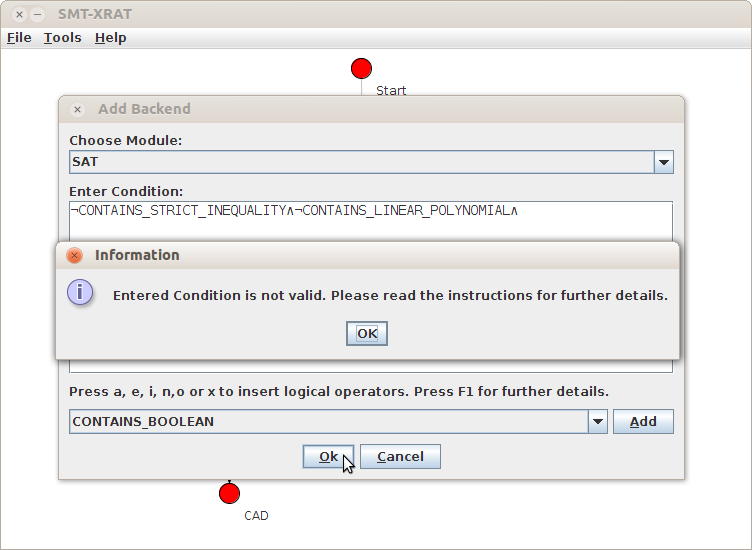
\includegraphics[width=0.9\textwidth]{graphics/smt-xrat_condition_wrong.png}
  \end{center}
  \caption{A wrong condition has been inputted by the user.}
  \label{fig:smt-xrat_condition_wrong}
\end{figure}

\subsubsection{Manipulating the strategy graph}
\label{sec:manipulating_the_strategy_graph}
Besides the capability of adding modules, the strategy graph pane gives the user also the possibility to remove and edit them subsequently.

The deletion of a single module implicates that all of its succeeding modules in the composition hierarchy will be removed as well. The strategy graph pane is only allowed to contain one single weakly connected graph. Furthermore, when deleting one or implicitly more modules, the priority values of all remaining modules might automatically be adjusted to comply the constraints of the priority values. However, the logical priority order remains untouched.

When editing modules, the same dialog window is displayed as for adding modules. The window components are already filled in with the attributes of the corresponding module. However, priority values are not manipulated via this dialog window. As said before, priority values are automatically assigned, when a module is created, and they are displayed alongside the edges. The user can manually change the priority order by pushing the priority value of a lower prioritized module in front of the priority value of a higher prioritized one. The user achieves this by using the mouse pointer to draw a dashed arrow from the edge label of that lower prioritized module to the edge label of the higher prioritized module, as it is illustrated by Figure \ref{fig:smt-xrat_priority_a}. Afterwards the lower prioritized module will have a higher priority than the other one. The priority values of the modules might just be swapped. If this is not possible, the priority values of the modules and of their 
preceding modules are adjusted automatically, so that as a result, the newly prioritized module will be ordered logically before the other one. The adaptation of the priority values is emphasized by Figure \ref{fig:smt-xrat_priority_b}. This mechanism has been implemented not only to offer a fast way of subsequently changing priority values, but also to picture the actions of the user even more.
\begin{figure}
  \begin{center}
    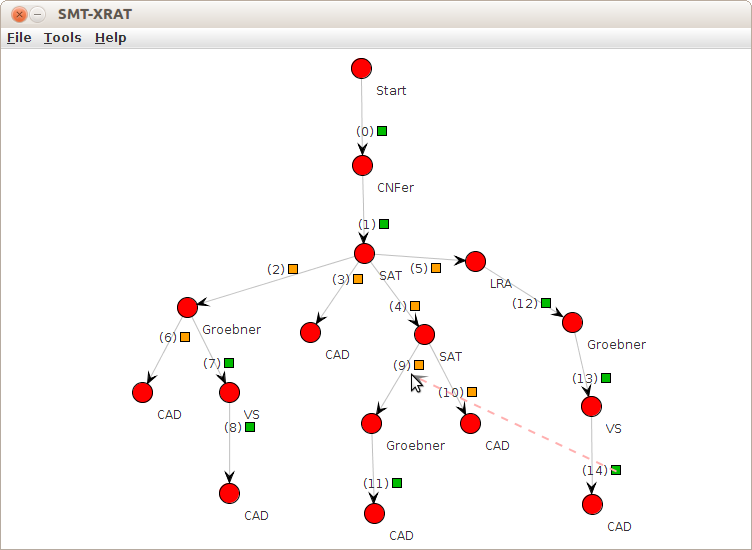
\includegraphics[width=0.9\textwidth]{graphics/smt-xrat_priority_a.png}
  \end{center}
  \caption{Priority values before changes are set.}
  \label{fig:smt-xrat_priority_a}
\end{figure}

\begin{figure}
  \begin{center}
    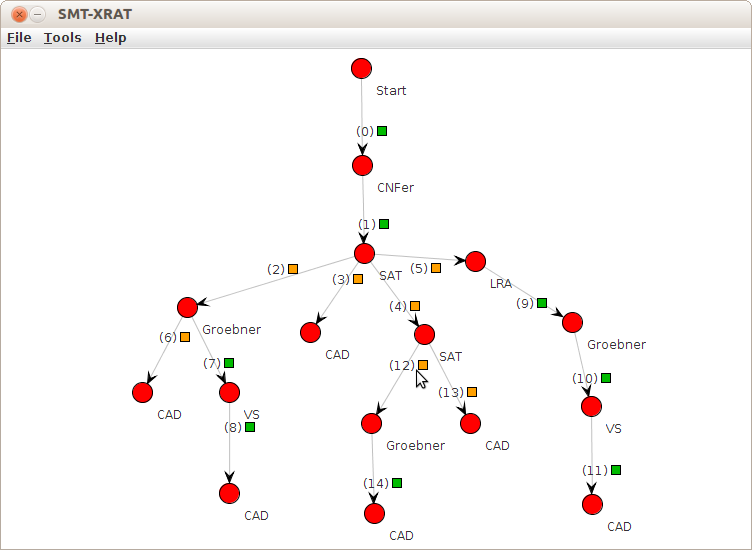
\includegraphics[width=0.9\textwidth]{graphics/smt-xrat_priority_b.png}
  \end{center}
  \caption{Intentionally changed and automatically adapted priority values.}
  \label{fig:smt-xrat_priority_b}
\end{figure}

Note that graph elements or even a group of graph elements can be positioned freely on the strategy graph pane anytime after there creation.

\subsection{Further functionalities}
\label{sec:further_functionalities}
Further features of the GUI are reached through the menu bar. The most important and also necessary functionality is the management of strategy graphs inside the SMT-RAT source code. It is not sufficient to design a strategy graph on the pane. Its underlying data structure also needs to be translated into source code, which must then be integrated into SMT-RAT. To export a currently modeled strategy graph, the user simply needs to open the corresponding dialog window and choose a name, Figure \ref{fig:managing_smt_solvers} shows an example for exporting the current strategy graph and naming it \emph{SMT\_XRAT}. The GUI will then fulfill the translation and integration process. The same dialog window also lists all existing strategy graphs, which are currently integrated in the source code, and gives the opportunity to delete them separately. This can be seen for the existing strategy graph \emph{NRATSolver} of the example.

The remaining features hold by the menu bar are not mandatory, but improve the creation process and usability. For example, the GUI allows the user to save the current strategy graph into an XML file. This file can then be opened again for later editing or it can be exchanged with another user. Another practical feature is the ability to save a screen shot of the strategy graph pane into an image file. Such image files can be used to discuss strategy graphs, when it is not desired to run the GUI. For this purpose, it could be attached into an email or included into a presentation, for instance.
\begin{figure}
  \begin{center}
    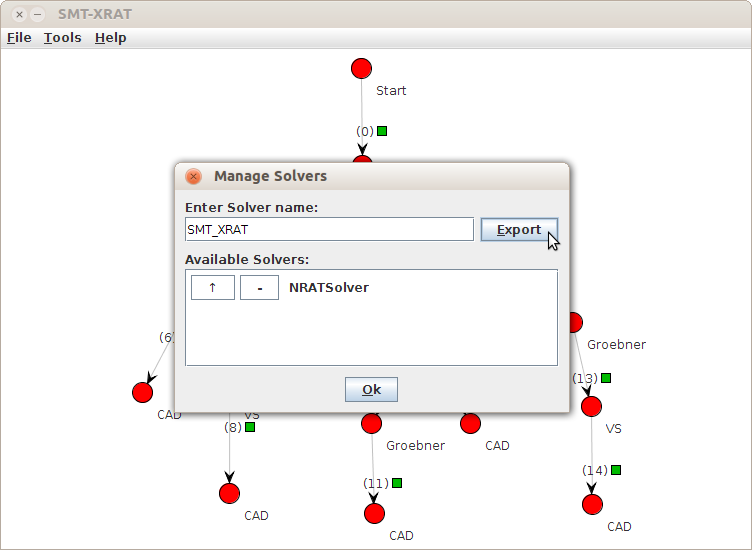
\includegraphics[width=0.9\textwidth]{graphics/smt-xrat_manage_solvers.png}
  \end{center}
  \caption{Managing SMT solvers in the SMT-RAT source code.}
  \label{fig:managing_smt_solvers}
\end{figure}





\end{document}
